\clearpage
\subsubsection{Numerical verification at small intervals}
\label{sec:num-ising-small}
At $y=1/2$, the analytical results above predict
$\alpha=2$ and $c_0^{\rm CFT}=\pi^2/48$ for the four directions
involving $\sigma$, and $\alpha=4$ and
$c_0^{\rm CFT}=2\pi^4/15$ for $I\leftrightarrow\varepsilon$.
Figure~\ref{fig:num-ising-small} and
Table~\ref{tab:num-ising-small} test these two distinct powers.
On $x\leq0.02$, the free exponents are about $2.0001$ for
$I\leftrightarrow\sigma$, $3.9934,3.9861$ for
$I\leftrightarrow\varepsilon$, and $2.0238,2.0176$ for
$\sigma\leftrightarrow\varepsilon$. A separate narrower-window
check at $x\leq0.001$ gives $1.999324,1.999296$ for the latter
two directions, without imposing the predicted exponent. This
illustrates why a finite-window effective power need not equal
its asymptotic value.

The two-term model uses the powers $\alpha,\alpha+2$.
It improves both leading-amplitude accuracy and omitted-size
prediction in all six directions. Its leading-amplitude errors
are below $0.82\%$ for $I\leftrightarrow\varepsilon$ and below
$0.045\%$ for the remaining directions. The two complete supplied
sixth-order coefficients provide a more stringent test:
\begin{align}
 c_1^{\rm CFT}(I\mid\varepsilon)&=-8\pi^6/45,
 &\widehat c_1&=-170.71,\nonumber\\
 c_1^{\rm CFT}(\varepsilon\mid I)&=-8\pi^6/21,
 &\widehat c_1&=-355.38.
 \label{eq:num-ising-second}
\end{align}
The signed discrepancies are approximately $-0.122\%$ and
$-2.966\%$. Thus the data test the directional asymmetry of the
sixth-order term as well as the common leading power, while
retaining a measurable discrepancy in the reverse direction.
Figure~\ref{fig:num-ising-small-residual} shows the residuals;
the other fitted next coefficients have no complete analytical
value for comparison.
% Condensed from numerical/tables/ising_small_parameters.tex; numerical values copied without refitting.
\begin{table}[htbp]\centering\footnotesize
\setlength{\tabcolsep}{3.5pt}
\begin{tabular}{lrrrrrrr}\toprule
Direction & $\widehat\alpha$ & $C_{\rm free}$ & $c_0^{\rm CFT}$ & $c_0(F_1)$ & $c_0(F_2)$ & $c_1(F_2)$ & $\eta_0(F_2)$\\\midrule
$I\mid \sigma$ & 2.0001 & 0.20585 & 0.20562 & 0.20573 & 0.20571 & 0.083833 & 0.044771\\
$\sigma\mid I$ & 2.0001 & 0.20582 & 0.20562 & 0.20572 & 0.2057 & 0.069099 & 0.042877\\
$I\mid \varepsilon$ & 3.9934 & 12.491 & 12.988 & 12.83 & 12.883 & -170.71 & -0.80492\\
$\varepsilon\mid I$ & 3.9861 & 12.07 & 12.988 & 12.77 & 12.882 & -355.38 & -0.81263\\
$\sigma\mid \varepsilon$ & 2.0238 & 0.23069 & 0.20562 & 0.2089 & 0.20565 & 12.604 & 0.017273\\
$\varepsilon\mid \sigma$ & 2.0176 & 0.22393 & 0.20562 & 0.20806 & 0.20566 & 9.3133 & 0.022414\\
\bottomrule\end{tabular}
\caption{Ising small-interval fits on $0<x\leq0.02$, with 1255 geometries per direction. The free fit is $C_{\rm free}x^{\widehat\alpha}$; $F_1,F_2$ impose the powers in Table~\ref{tab:num-powers}. All amplitudes include powers of $\pi$. The final column is the signed leading-amplitude discrepancy of $F_2$ in percent, Eq.~\eqref{eq:num-residuals}. The $c_1$ column gives a fitted next amplitude, not a theoretical prediction.}
\label{tab:num-ising-small}
\end{table}

\begin{figure}[p]\centering
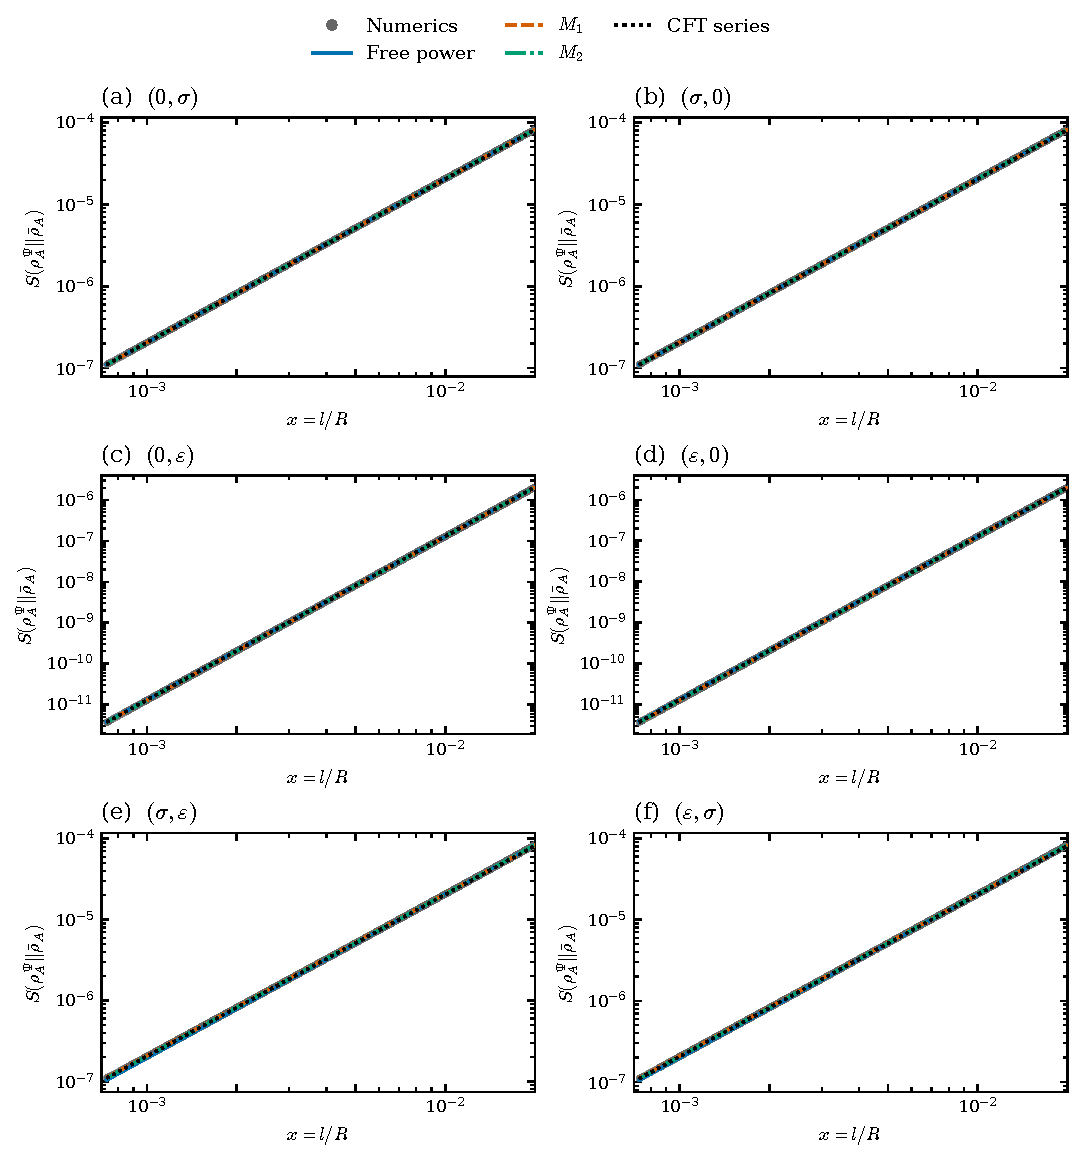
\includegraphics[width=.94\linewidth,height=.74\textheight,keepaspectratio]{figs/ising_small_fit_window_value.pdf}
\caption{Ising small-interval $D^A_{a\mid b}$ for all six ordered pairs. All 1255 displayed geometries per direction lie in the fitting window $0<x\leq0.02$, with $\ell=6,\ldots,10$. Both axes are logarithmic. Gray circles denote numerical data, using the same shape and color for every subsystem length. Blue solid, orange dashed, and green dash--dotted curves denote the free fit, $F_1$, and $F_2$; black dotted denotes the parameter-free CFT series. All curves are restricted to the fitting window.}
\label{fig:num-ising-small}
\end{figure}

\begin{figure}[p]\centering
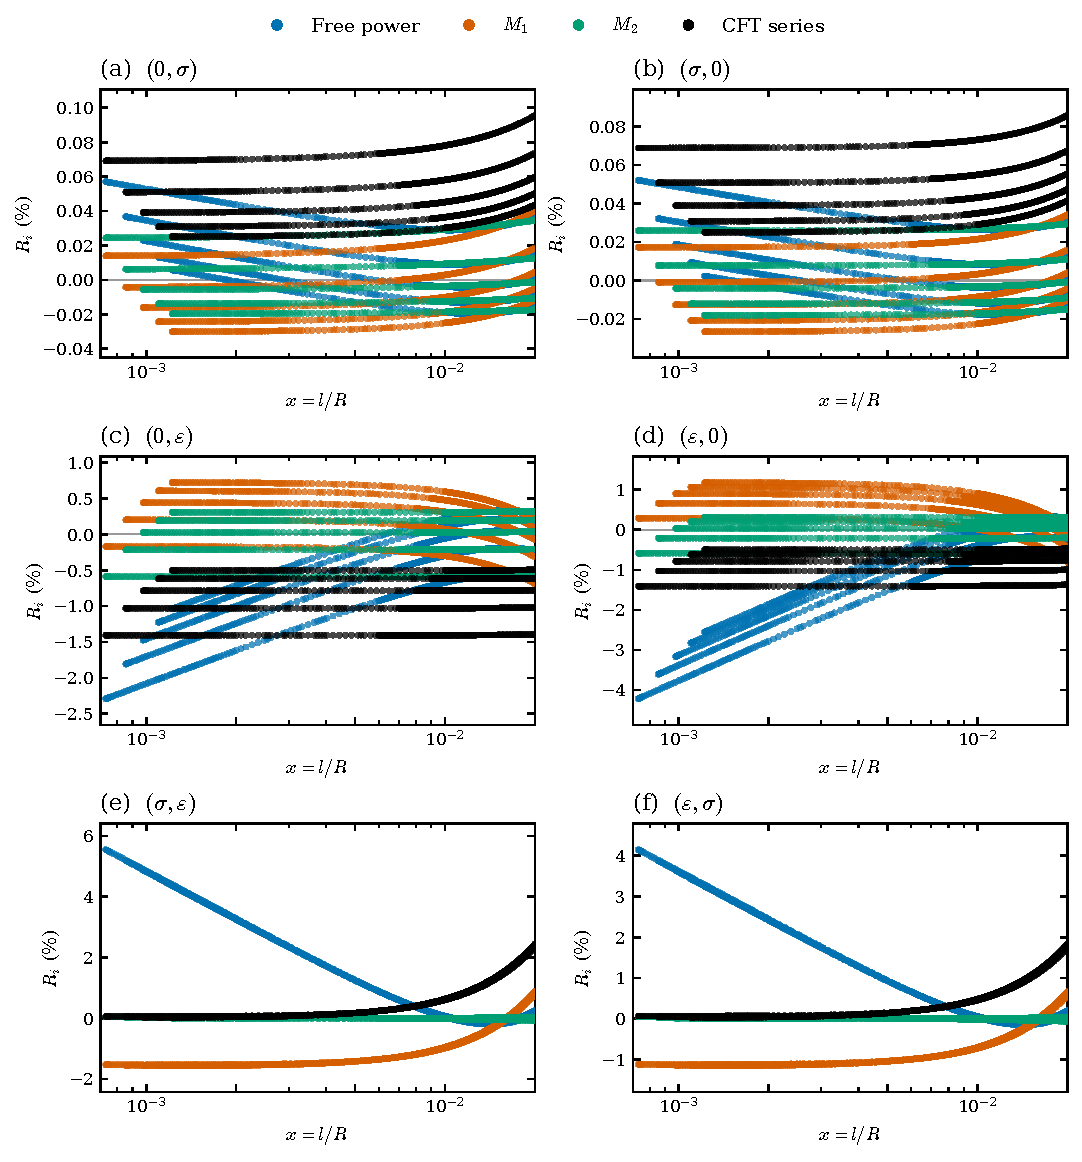
\includegraphics[width=.94\linewidth,height=.74\textheight,keepaspectratio]{figs/ising_small_fit_window_residual.pdf}
\caption{Signed percentage residuals $100[q-M]/q$ for Fig.~\ref{fig:num-ising-small}, with $q=D^A$. The residual ordinate is linear and the fraction axis logarithmic. Only the 1255 fitted geometries per direction at $0<x\leq0.02$ are shown. All subsystem lengths $\ell=6,\ldots,10$ use circular markers; colors identify models and are identical across lengths. Blue, orange, green, and black denote the free fit, $F_1$, $F_2$, and the parameter-free CFT series.}
\label{fig:num-ising-small-residual}
\end{figure}

\clearpage

\subsubsection{Numerical verification at large intervals}
\label{sec:num-ising-large}
The different mixing OPEs predict deficit powers
$\beta=1/4,2,1/4$ for $I\leftrightarrow\sigma$,
$I\leftrightarrow\varepsilon$, and
$\sigma\leftrightarrow\varepsilon$, respectively.
Their leading amplitudes are
\begin{equation}
 B_\sigma=\frac{\pi^{3/4}\Gamma(9/8)}{4\Gamma(13/8)}
 \simeq0.61965,\qquad \frac{\pi^2}{3},\qquad
 \frac{B_\sigma}{4}.
 \label{eq:num-ising-large-leading}
\end{equation}
The factor of four between the spin channels tests the squared
mixing OPE coefficient. Figure~\ref{fig:num-ising-large} and
Table~\ref{tab:num-ising-large} compare these predictions with
the independently evaluated deficits.

On $\ep\leq0.002$, $I\leftrightarrow\sigma$ has an effective
free power of about $0.26465$, approximately $5.86\%$ above $1/4$.
Including the allowed $\ep^{1/2}$ term reduces the leading-amplitude
error from $+5.44\%$ in $F_1$ to about $-0.81\%$ in $F_2$.
For $\sigma\mid\varepsilon$ and $\varepsilon\mid\sigma$, the
free powers are $0.25058$ and $0.25544$ and the $F_2$
leading-amplitude errors are $+0.67\%$ and $-0.81\%$.
For $I\leftrightarrow\varepsilon$, the free powers
$1.9985,2.0013$ are close to two, and the $F_2$ amplitudes differ
from $\pi^2/3$ by $-0.025\%,+0.118\%$.

All six directions improve in both leading-amplitude accuracy
and omitted-size prediction with $F_2$.
Figure~\ref{fig:num-ising-large-residual} makes the remaining
deviations visible. These fits support the leading fractional
powers and OPE amplitudes, but the fixed powers of $F_2$ are inputs
to that fit, and its next coefficients are numerical estimates.
The finite-window free exponent in the vacuum--spin channel
remains distinguishable from $1/4$.
% Condensed from numerical/tables/ising_large_parameters.tex; numerical values copied without refitting.
\begin{table}[htbp]\centering\footnotesize
\setlength{\tabcolsep}{3.5pt}
\begin{tabular}{lrrrrrrr}\toprule
Direction & $\widehat\beta$ & $C_{\rm free}$ & $c_0^{\rm CFT}$ & $c_0(F_1)$ & $c_0(F_2)$ & $c_1(F_2)$ & $\eta_0(F_2)$\\\midrule
$I\mid \sigma$ & 0.26465 & 0.71994 & 0.61965 & 0.65339 & 0.61463 & 0.20243 & -0.81098\\
$\sigma\mid I$ & 0.26465 & 0.71995 & 0.61965 & 0.65339 & 0.61462 & 0.20245 & -0.81139\\
$I\mid \varepsilon$ & 1.9985 & 3.2548 & 3.2899 & 3.2861 & 3.289 & -1070.2 & -0.024918\\
$\varepsilon\mid I$ & 2.0013 & 3.3242 & 3.2899 & 3.2964 & 3.2938 & 959.21 & 0.11818\\
$\sigma\mid \varepsilon$ & 0.25058 & 0.15691 & 0.15491 & 0.15631 & 0.15595 & 0.0018716 & 0.67037\\
$\varepsilon\mid \sigma$ & 0.25544 & 0.16288 & 0.15491 & 0.15712 & 0.15365 & 0.018087 & -0.81285\\
\bottomrule\end{tabular}
\caption{Ising large-interval fits on $0<\ep\leq0.002$, with 260 geometries per direction. The free fit is $C_{\rm free}\ep^{\widehat\beta}$; $F_1,F_2$ impose the powers in Table~\ref{tab:num-powers}. All amplitudes include powers of $\pi$. The final column is the signed leading-amplitude discrepancy of $F_2$ in percent, Eq.~\eqref{eq:num-residuals}. The $c_1$ column gives a fitted next amplitude, not a theoretical prediction.}
\label{tab:num-ising-large}
\end{table}

\begin{figure}[p]\centering
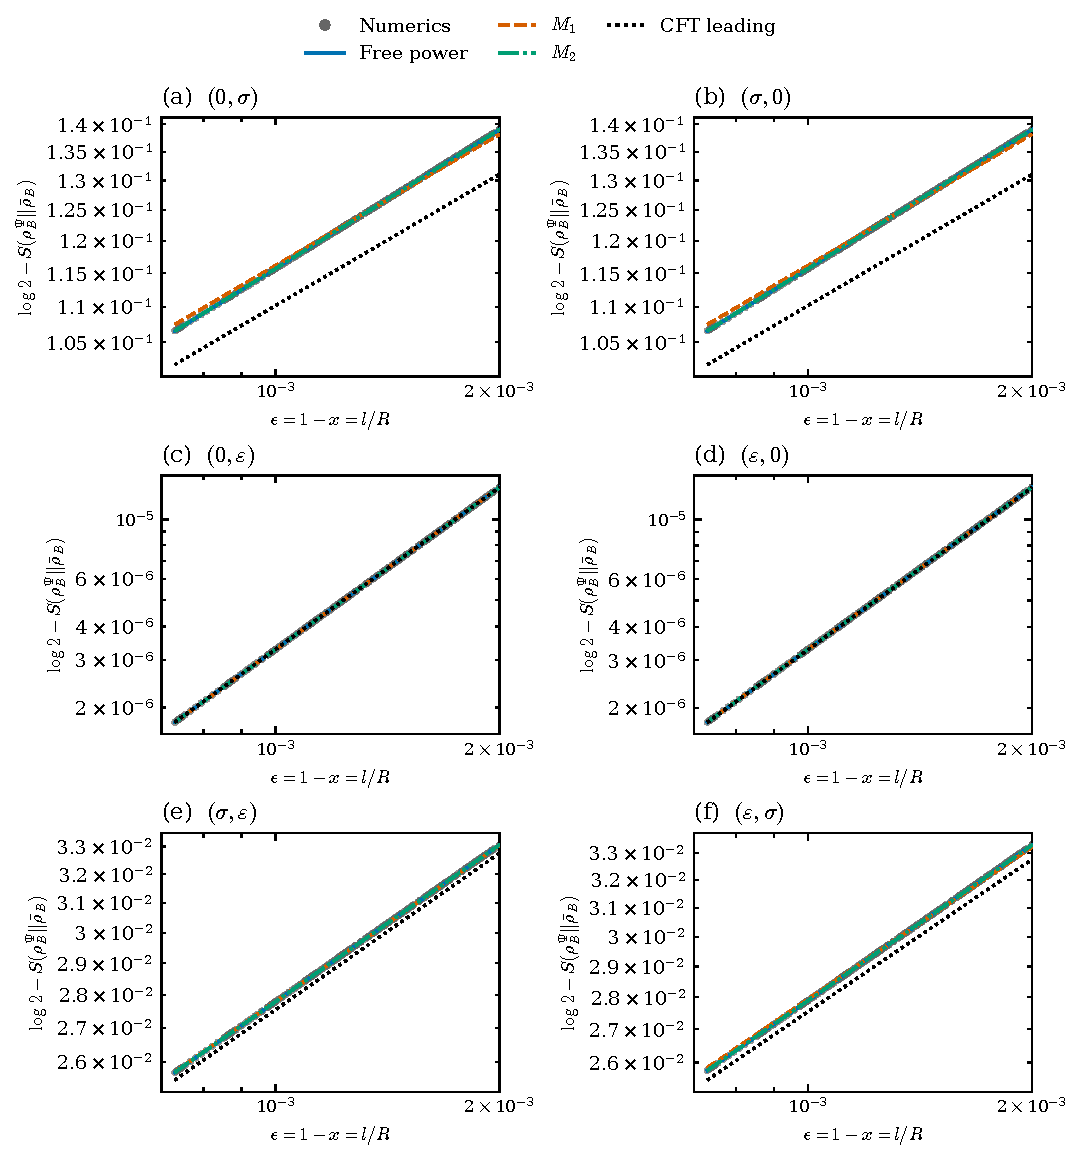
\includegraphics[width=.94\linewidth,height=.74\textheight,keepaspectratio]{figs/ising_large_fit_window_value.pdf}
\caption{Ising large-interval $\delta_{a\mid b}=\log2-D^B_{a\mid b}$ for all six ordered pairs. All 260 displayed geometries per direction lie in the fitting window $0<\ep\leq0.002$, with $\ell=6,\ldots,10$. Both axes are logarithmic. Gray circles denote numerical data, using the same shape and color for every subsystem length. Blue solid, orange dashed, and green dash--dotted curves denote the free fit, $F_1$, and $F_2$; black dotted denotes the parameter-free CFT leading term. All curves are restricted to the fitting window. The horizontal label $y$ denotes the complement fraction $\ep=1-x_B=\ell/N$, while the mixing probability is fixed at $1/2$.}
\label{fig:num-ising-large}
\end{figure}

\begin{figure}[p]\centering
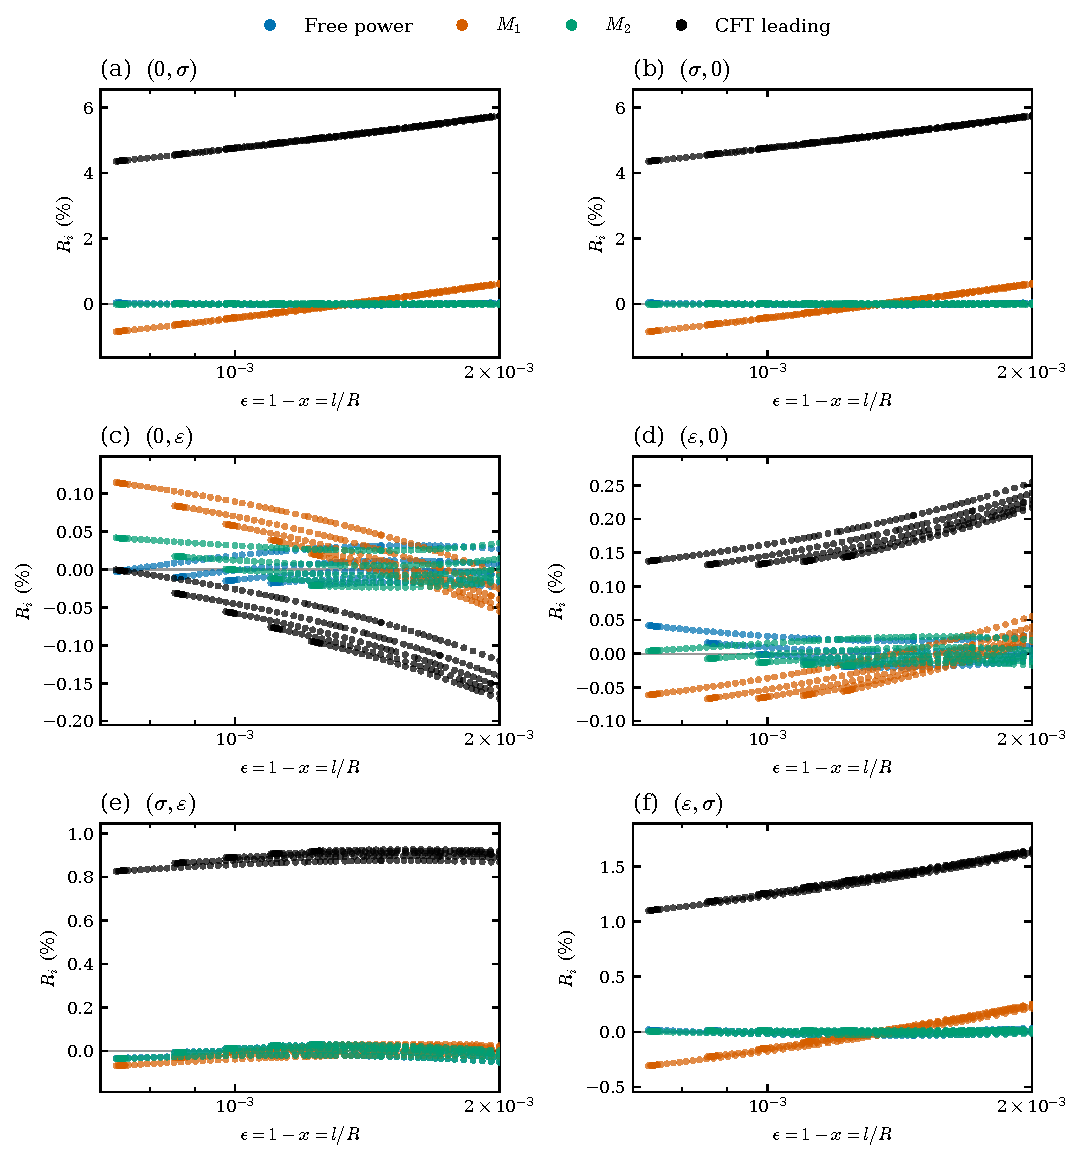
\includegraphics[width=.94\linewidth,height=.74\textheight,keepaspectratio]{figs/ising_large_fit_window_residual.pdf}
\caption{Signed percentage residuals $100[q-M]/q$ for Fig.~\ref{fig:num-ising-large}, with $q=\delta$. The residual ordinate is linear and the fraction axis logarithmic. Only the 260 fitted geometries per direction at $0<\ep\leq0.002$ are shown. All subsystem lengths $\ell=6,\ldots,10$ use circular markers; colors identify models and are identical across lengths. Blue, orange, green, and black denote the free fit, $F_1$, $F_2$, and the parameter-free CFT leading term. The horizontal label $y$ denotes the complement fraction $\ep=1-x_B=\ell/N$, while the mixing probability is fixed at $1/2$.}
\label{fig:num-ising-large-residual}
\end{figure}

\clearpage
